\documentclass{article}
\usepackage[margin=.9in]{geometry}
\usepackage[dvipsnames]{xcolor}
\usepackage{amsmath}
\usepackage{amssymb}
\usepackage{amsthm}
\usepackage{tikz}
\usepackage{mathrsfs}
\usepackage{indentfirst}
\usepackage{float}
\newtheorem*{claim}{Claim}
\newtheorem*{lemma}{Lemma}
\newtheorem*{poof}{Proof}
\title{Final Portfolio}
\author{Christopher Hunt}
\date{}
\usepackage{graphicx} 
\usepackage{fancyhdr}

\begin{document}
\pagestyle{fancy}
\fancyhf{}
\rfoot{MTH 231}
\lfoot{Christopher Hunt}
\lhead{Final Portfolio}
\rhead{\thepage}
\maketitle

\section*{Reflective Introduction}
The purpose of this portfolio is to showcase my understanding of the major contents covered in this course. Throughout the course, we explored seven core sections, each contributing to my development as a mathematician. To demonstrate my understanding of set theory, I chose question 25, which presented a variety of set theory concepts. This problem required knowledge of sets, subsets, set notation, and how to analyze relationships between different sets.

For propositional logic, I selected SQ-1, which tested my understanding of notation, statements, and predicates. Converting sentences into variable notation and applying negation were essential skills showcased in this problem.

To demonstrate my ability to prove statements directly, I chose problem 7, which provided a clear and straightforward example of a direct proof. Additionally, I included part b of question 7 and SQ-4 to showcase my work with indirect proofs. Problem 7b required me to apply proof by counterexample, while the lemma in SQ-4 employed proof by contradiction. Both problems demonstrated my proficiency in constructing logical arguments and applying different proof techniques.

For proofs by mathematical induction, I tackled the challenging question 22. This problem tested my ability to reason step-by-step and apply mathematical induction effectively. Similarly, SQ-8 on combinatorics proved to be an interesting and demanding problem that required careful wording and precise solutions.

In graph theory, I found the concepts of trees and spanning trees to be fundamental. SQ-11 specifically addressed these topics, allowing me to apply my knowledge of set theory and proofs to find solutions.

Moving on to my overall grade for the course, I am confident that I have met the learning objectives and excelled in my assignments. In addition to completing the homework and Daily Prep diligently, I took the initiative to review the material before class, making notes to enhance my understanding. Actively participating in class discussions and volunteering to present the daily prep problems further showcased my commitment to learning.

Overall, I have developed a solid understanding of all the topics covered in this course. I have gained valuable tools for proving statements and solving problems, which will undoubtedly benefit me in future mathematical endeavors. With my dedication and the quality of work I have produced, I believe I have earned an 'A' for my performance in this course.


\newpage
\section*{Set Theory}
\section*{25. Let $A$, $B$, and $C$ be sets.}
\subsection*{a. Suppose that $A \subseteq B$ and $B \subseteq C$. Does this mean that $A \subseteq C$?}
\begin{claim}
    If $A \subseteq B$ and $B \subseteq C$, then $A \subseteq C$.
\end{claim}
\begin{poof}
    Assume $A \subseteq B$ and $B \subseteq C$ is true. By the definition of a subset we can state that every element $x$ in $A$ is an element in $B$ and every element $y$ in $B$ is an element of $C$. This can be visualually demosntrated using this Venn diagram:
    \begin{center}
        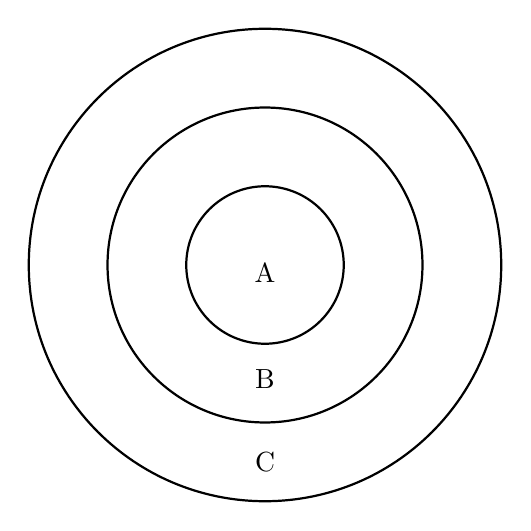
\begin{tikzpicture}[thick]
          % Draw outer circle (C)
          \draw (0,0) circle (3cm);
          \node[text=black] at (0,-2.5cm) {C};
          % Draw middle circle (B)
          \draw (0,0) circle (2cm);
          \node[text=black] at (0,-1.45cm) {B};
          % Draw inner circle (A)
          \draw (0,0) circle (1cm);
          \node[text=black] at (0,-.10cm) {A};
        \end{tikzpicture}
    \end{center}
    Since, every element of $B$ must be in $C$ and every element of $A$ must be in $B$ it follows that every element of $A$ must also be in $C$. Therefore, $A \subseteq C$ is true and the  from that the original claim is true. \\
    \qed
\end{poof}


\subsection*{b. Suppose that $A \in B$ and $B \in C$. Does this mean that $A \in C$? Give an example to prove that this does NOT always happen.}
\begin{claim}
    If $A \in B$ and $B \in C$, then $A \in C$.
\end{claim}
\begin{poof}
    For this claim to be false we must find a case where $A \in B$ and $B \in C$ is true but $A \in C$ is false. Consider the following sets, $A$, $B$, and $C$:
    \begin{align*}
        A &= \{1,2\}\\
        B&= \{A,3\}\\
        C&=\{B,4\}
    \end{align*}  
    These sets fullfil the antecedent of the claim above. They can also be expressed like:
    \begin{align*}
        A &= \{1,2\}\\
        B&= \{\{1,2\},3\}\\
        C&=\{\{\{1,2\},3\},4\}
    \end{align*}
    Viewing the expressions this way we can see that A is an element of an element of $C$ but not directly an element itself, which violates the claim that $A$ is an element of $C$ if $A$ is an element of $B$ and $B$ is an element of $C$. Therefore the claim is not always true.\\  
    \qed
\end{poof}
\newpage
\section*{Propositional Logic}
\section*{SQ-1. The notation $\exists !$ means ``there exists a unique.'' For example, ``$\exists !$ x such that x is prime and x is even'' means that there is one and only one even prime number. Suppose that P(x) is a predicate and D is the domain of discourse for x.}
\subsection*{a. Rewrite the statement ``$\exists ! x \in D:P(x)$'' without using the symbol $\exists !$.}
Let:
\[Q(x,y) = \text{y is x}\]
The statement ``$\exists ! x \in D:P(x)$'' can be rewritten as:
\[\text{There exists some x in D such that P(x), and, for all y in D, if P(y), then y is x.}\]
\[\exists x \in D : (P(x) \wedge (\forall y \in D : (P(y) \rightarrow Q(x,y)))) \]
\subsection*{b. Write (and simplify) a negation of the statement ``$\exists ! x \in D:P(x)$.'' What does it mean in words?}

The negation of the statement above is:
\[\text{For all x in D ~P(x), or, there exists some y in D such that, P(y) and y is not x}\]
Symbolically this can be done using de Morgan's Law:
\[\neg (\exists x \in D : (P(x) \wedge (\forall y \in D : (P(y) \rightarrow (y = x))))) \equiv \; \forall x \in D : (\neg P(x) \vee (\exists y \in D : (P(y) \wedge \neg Q(x,y))))\]
\newpage
\section*{Direct Proof}
\section*{7. Consider the statement: for all integers $a$ and $b$, if $a$ is even and $b$ is a multiple of 3, then $ab$ is a multiple of 6.}
Let us begin by defining our terms.
\begin{align*}
    &\text{Let: } a,b,n,m\in\mathbb{Z} \\
    &P(a,n) = ``a = 2n'' \quad \text{(by the definition of even numbers from class)} \\
    &Q(b,m) = ``3|b=m'' \text{ or } ``b=3m'' \\
    &R(a,b,n,m)= ``6|ab=nm'' \text{ or } ``ab = 6(nm)''
\end{align*}
\subsection*{a. Prove the statement. What sort of proof are you using?}
This claim will be proven using a Direct Proof.
\begin{claim}
For all integers $a$ and $b$, if $P$ and $Q$ are true, then $R$ is true. That is, $\forall a, b \in \mathbb{Z} (P \wedge Q \rightarrow R)$.
\end{claim}

\begin{poof}
Suppose $P$ and $Q$ are true. Consider the product of $a$ and $b$:
\begin{align*}
    ab &= (2n)(3m) \\
       &= 6(nm)
\end{align*}
Since $a$, $b$, $n$, and $m$ are all integers, and integers are closed under multiplication, we can conclude that the product of $ab$ is divisible by $6$. Therefore, the claim is true. \\
\qed\end{poof}


\subsection*{b. State the converse. Is it true? Prove or disprove.}
Now consider the converse claim.
\begin{claim}
For all integers $a$ and $b$, if $R$ is true, then $P$ and $Q$ are true. That is, $\forall a, b \in \mathbb{Z} (R \rightarrow P \wedge Q)$.
\end{claim}

\begin{poof}
Suppose $R$ is true. For the statement to be true $a$ must be even and $b$ a multiple of 3. To disprove this claim we need to show that there exists a product of $a$ and $b$ that is a multiple of 6 where either $a$ is not even or $b$ is not a multiple of 3. Consider this counterexample:
\[\text{Let: } a = 6 \text{ and } b = 2 \]
\begin{align*}
       ab &= 6(2) \\
       &= 12 \\
\end{align*}
Since the product of $a$ and $b$ is a multiple of 6, and $b$ is not a multiple of 3 there exists a case where the statement $R$ is true but the implication $P \wedge Q$ is false. Therefore, the converse claim is false. \\
\qed\end{poof}
\newpage
\section*{Indirect Proof}
\section*{SQ-4. For all sets $A$ and $B$,}
\subsection*{a. Prove that $A$ is a subset of $B$ if and only if $B^c$ is a subset of $A^c$.}
To begin this proof we must start with proving that the cardinality of a subset of a set is less than or equal to the cardinality of the set itself.
\begin{claim}
    $A \subseteq B \rightarrow |A| \leq |B|$
\end{claim}
\begin{lemma}
    To prove this we will use proof by contradiction. Suppose the claim were not the case, then $A \subseteq B \wedge |A| > |B|$. This means that there must be at least one element in $A$ that is not also in $B$, in order for this to be true $A$ could not be a subset of $B$ by the definition of subsets. Therefore the claim is true by contradiction.
\end{lemma}
    
\begin{claim}
    $A \subseteq B \leftrightarrow B^c \subseteq A^c$
\end{claim}
\begin{poof}
    This bidirectional claim can be broken down into two implications:
    \begin{align*}
        1.&\;A\subseteq B \rightarrow B^c\subseteq A^c\\
        2.&\;B^c\subseteq A^c \rightarrow A\subseteq B
    \end{align*}
    Let's assume the antecedant of claim one to be true. That is $A$ is a subset of $B$.
    \begin{figure}[H]
    \centering
        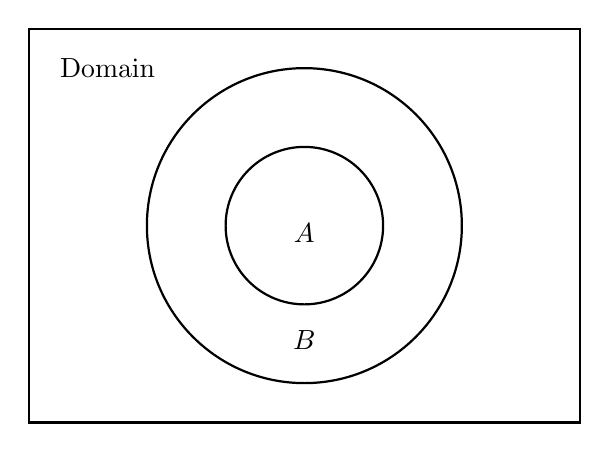
\begin{tikzpicture}[thick]
          % Draw box
          \draw (-3.5cm,-2.5cm) rectangle (3.5cm,2.5cm);
          \node[text=black] at (-2.5cm, 2) {Domain};
          % Draw middle circle (B)
          \draw (0,0) circle (2cm);
          \node[text=black] at (0,-1.45cm) {$B$};
          % Draw inner circle (A)
          \draw (0,0) circle (1cm);
          \node[text=black] at (0,-.10cm) {$A$};
        \end{tikzpicture}
    \end{figure}
    Now consider $B^c$ and $A^c$ which are the areas in the domain which are outside the corresponding sets of $A$ and $B$. Since every element of $A$ is in $B$ we know that $A$ has less than or equal to the same number of elements as $B$ by Lemma 1. Taking their compliment we know that $B^c$ is less than or equal to $A^c$ and since all the elements in $A$ are also in $B$, we know that any element which is not in $B$ must also not be in $A$ which meets the definition of a subset. Therefore the implication is true.

    Now Let's assume the antecedent of the second claim is true. That is every element not in $B$ is also not in $A$.
    \begin{figure}[H]
        \centering
            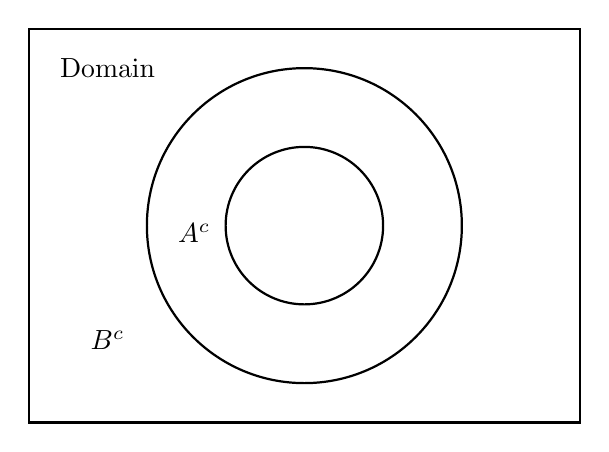
\begin{tikzpicture}[thick]
              % Draw box
              \draw (-3.5cm,-2.5cm) rectangle (3.5cm,2.5cm);
              \node[text=black] at (-2.5cm, 2) {Domain};
              % Draw middle circle (B)
              \draw (0,0) circle (2cm);
              \node[text=black] at (-2.5cm,-1.45cm) {$B^c$};
              % Draw inner circle (A)
              \draw (0,0) circle (1cm);
              \node[text=black] at (-1.4cm,-.10cm) {$A^c$};
            \end{tikzpicture}
        \end{figure}
    Due to this fact every element not in $A^c$ must also not be in $B^c$, that is every element in $A$ is also in $B$. Therefore the second claim holds. Since both claims are true then the original claim is also true. \\
    \qed\end{poof}


\subsection*{b. Prove that if $A$ is a subset of $B$ and $B$ is a subset of $A$, then $A=B$.}
\begin{claim}
    $A \subseteq B \wedge B \subseteq A \rightarrow A = B$
\end{claim}
\begin{poof}
    Assume that $A \subseteq B$ and $B \subseteq A$ are both true. That is, every element of $A$ is an element of $B$ and every element of $B$ is an element of $A$. Consider some arbitrary element $x$ in the set $A$, this element will be in set $B$. Now, consider some other arbitrary element $y$ in set $B$, this element will be in set $A$ as well. Since there are no elements that can be found in $A$ that are not in $B$ and no elements that can be found in $B$ that are not in $A$, therefore $A$ and $B$ contain exactly the same elements. Therefore the claim is true. \\ 
    \qed\end{poof}
\newpage
\section*{Proof By Mathematical Induction}
\section*{22. Suppose that a particular real number 
 has the property that $x+\frac{1}{x}$ is an integer. Prove that $x^n+\frac{1}{x^n}$ is an integer for all natural numbers.}

\begin{claim}
     $x^n+\frac{1}{x^n}$ is an integer for all natural numbers.
     \[\forall n \in \mathbb{N}, x^n +\frac{1}{x^n}\text{ \emph{is an integer}}\]
\end{claim}
\begin{poof}
     Let's begin by considering the base case where n = 1.
    \begin{align*}
         x^1+&\frac{1}{x^1}\\         x+&\frac{1}{x}
    \end{align*}
    Since $x+\frac{1}{x}$ is assumed to be an integer we can state that the claim where n=1, is true.
    \\
    
    \noindent Now let us assume for all integers from 0 to k the claim holds true. Since we know that integers have closure under multiplication if we multiplied the integer $x^k+\frac{1}{x^k}$ by $x+\frac{1}{x}$ the product will be an integer. Consider the expansion of this product equals some integer j.
    \begin{align*}
        (x^k+\frac{1}{x^k})(x+\frac{1}{x})=&\,j\\
        x^{k}x+\frac{x^k}{x}+\frac{x}{x^k}+\frac{1}{x^{k}x}=&\,j\\
        x^{k+1}+\frac{1}{x^{k+1}}+x^{k-1}+\frac{1}{x^{k-1}}=&\,j\\
    \end{align*}
    Since we are assuming that the claim holds for all values up to k, it will then hold true for $k-1$. We can replace $x^{k-1}+\frac{1}{x^{k-1}}$ for some integer $m$
    \begin{align*}
        x^{k+1}+\frac{1}{x^{k+1}}+x^{k-1}+\frac{1}{x^{k-1}}=&\,j\\
        x^{k+1}+\frac{1}{x^{k+1}}+m=&\,j
    \end{align*}
    Since we know that both j and m are integers and integers are closed under addition the sum of $x^{k+1}+\frac{1}{x^{k+1}}$ must also be an integer. Therefore by strong induction, the claim is true.
    \\
    \qed\end{poof}
\newpage
\section*{Combinatorics}
\section*{SQ-8. Determine the number of five-card poker hands that contain three queens. How many of them contain, in addition to the three queens, another pair of cards?}

To find the number of five-card poker hands that contain three queens we can consider two different choice cases. In the first case, out of the four queens available in the deck 3 are chosen, then from the remaining 48 cards we choose two.
\[\binom{4}{3}*\binom{48}{2}\]
In the second case, we choose the frist three queens, then from the remaining 48 we choose 1 and then we get the fourth queen free.
\[\binom{4}{3}*\binom{48}{1}*\binom{1}{1}\]
To find the total number of combinations, we add these two values together:
\[\binom{4}{3}*\binom{48}{2}+\binom{4}{3}*\binom{48}{1}\binom{1}{1} = 4704\]
There are $4704$ possible poker hands that contain at least three queens.
\\
Next, if we want to find the possible hands with three queens and two pairs we must first choose three of the four queens, then draw one of the remaining forty-eight, then from the remaining three suits of that previous card, draw one. This total must then be divided by half since order doesn't matter and we need to remove the double counted pairs.
\[\frac{\binom{4}{3}*\binom{48}{1}*\binom{3}{1}}{2!} = 288\]
There are $288$ possible full house poker hands with three queens!
\newpage
\section*{Graph Theory}
\section*{SQ-11. Suppose $G$ is a connected graph and $T$ is a cycle-free subgraph of $G$. Suppose also that if any edge $e$ of $G$ that is not in $T$ is added to $T$, the resulting graph contains a cycle. Prove that $T$ is a spanning tree for $G$}
\begin{claim}
    $T$ is a spanning tree for $G$
\end{claim}
\begin{poof}
    First, we will show that T is a tree. Since T is a cycle-free subgraph of G, it is by definition acyclic. Now we need to prove that T is connected. Suppose T is not connected, which means there are two sets of vertices in T that are not adjacent to each other. Let's call these sets A and B. Since G is a connected graph, there exists at least one edge (u, v) in G that connects a vertex in set A to a vertex in set B. Adding this edge to T would create a cycle, contradicting the given condition that any edge not in T would create a cycle. Therefore, T must be connected, and hence a tree.

    Next, we will show that T spans all the vertices of G. Since T is a subgraph of G, it contains a subset of vertices from G. To prove that T spans all the vertices of G, we need to show that every vertex in G is also a vertex in T. Suppose there exists a vertex v in G that is not in T. Since G is a connected graph, there exists a path in G from any vertex u in T to vertex v. Along this path, there must be an edge e that is not in T. However, adding this edge e to T would create a cycle, which contradicts the given condition. Therefore, every vertex in G is also a vertex in T, and T spans all the vertices of G.
    
    Based on the above arguments, we have shown that T is a connected, acyclic subgraph of G that spans all the vertices of G. Therefore, T is a spanning tree for G.\\
\qed\end{poof}
\end{document}